\documentclass[%
%%%%%		PDFTex verwenden
pagesize=pdftex,
%%%%%   Language
german,
%%%%%   Paper size
a4paper,
%%%%%		Schriftgröße Standard 11
fontsize=11pt,
%%%%%   Get smaller borders and more space for writing
%%%%% ATTENTION be carefull with your binding! See scrbook manual! 
DIV=14,
%%%%%   Set the binding correction
BCOR=10mm,
%%%%%   Create smaler headlines
2.5headlines, 
%%%%%   Create small headings
headings=small, 
%%%%%   Use a titlepage
titlepage, 
%openbib,
%%%%%   Bibliography in Table of Contents with a chapter number
%bibliography=totocnumbered,
%%%%%   Bibliography in Table of Contents without a chapter number
bibliography=totoc,
%%%%%   Add the prefix "Appendix" to the apendix chapters
appendixprefix = true,
%%%%%   Use a twoside style
%%%%% ATTENTION oneside will change layout completely! Check this early!
twoside,
%open=any,
%oneside,
parskip=half,
]{scrbook}
%%%%%%%%%%%%%%%%%%%%%%%%%%%%%%%%%%%%%%%%%%%%%%%%%%%%%%%%%%%%%
%% INCLUDE PACKAGES
%%%%%%%%%%%%%%%%%%%%%%%%%%%%%%%%%%%%%%%%%%%%%%%%%%%%%%%%%%%%%
\usepackage[ngerman, german]{babel}
\usepackage[utf8]{inputenc}
\usepackage{graphicx}
\usepackage{color}
\usepackage{xcolor}
\usepackage[autooneside,automark]{scrpage2}
\usepackage[pdftex, pdfdisplaydoctitle=true, colorlinks, linktocpage, linkcolor=black, citecolor=black, urlcolor=black]{hyperref}
\usepackage{bookmark}
\usepackage{longtable,ltcaption}
\usepackage{wrapfig}
\usepackage{textcomp}
\usepackage{listings}
\usepackage{subfigure}
\usepackage{fancybox}
\usepackage{tabularx}
\usepackage[stable]{footmisc}
\usepackage[T1]{fontenc}
\usepackage{caption}
\usepackage{colortbl}
\usepackage{amssymb}
\usepackage[xindy,toc]{glossaries}
\usepackage[section]{placeins}
\usepackage{scala}
%%%%%%%%%%%%%%%%%%%%%%%%%%%%%%%%%%%%%%%%%%%%%%%%%%%%%%%%%%%%%
%% DOCUMENT DEFINITIONS
%%%%%%%%%%%%%%%%%%%%%%%%%%%%%%%%%%%%%%%%%%%%%%%%%%%%%%%%%%%%%
\newcommand{\docAuthor}{Tom Bocklisch}
\newcommand{\docAuthorMail}{tom.bocklischstudent.hpi.uni-potsdam.de}
\newcommand{\docTitle}{Eine Architektur für ein ereignisgesteuertes, webbasiertes Backend für Project-Zoom}
\newcommand{\docSupervisited}{Prof. Dr. Holger Giese, \\Thomas Beyhl, M.Sc. und\\ Gregor Berg}
\newcommand{\docCity}{Potsdam}
\newcommand{\docDate}{\today}
\newcommand{\docChair}{Systemanalyse und Modellierung}%System Analysis and Modeling Group}
\newcommand{\tete}[1]{\textit{#1}}
%%%%%%%%%%%%%%%%%%%%%%%%%%%%%%%%%%%%%%%%%%%%%%%%%%%%%%%%%%%%%
%% END OF DOKUMENT DEFINITIONS
%%%%%%%%%%%%%%%%%%%%%%%%%%%%%%%%%%%%%%%%%%%%%%%%%%%%%%%%%%%%%
\captionsetup{format=plain,labelfont=bf,labelsep=endash,justification=RaggedRight}%,indention=1cm}
%globale Wörtertrennung
\hyphenation{Graph-struk-tur Story-patterns Story-pattern}

\newcommand{\appendixChapter}[1]{\chapter{#1}\setcounter{page}{1}}

\def\TReg{\textsuperscript{\textregistered}}

%\zitat{quotation}
\newcommand{\zitat}[1]{
 \begin{quote}
  \fboxsep5mm
  \shadowbox{
  \begin{minipage}{0.8\textwidth}
    #1
  \end{minipage}}
\end{quote}}

%\begriff{caption}{quotation or definition}
\newcommand{\begriff}[2]{
  \begin{quote}
  \fboxsep5mm
  \shadowbox{
  \begin{minipage}{0.8\textwidth}
   \begin{center}\textbf{#1}\end{center}
   \bigskip
   #2
  \end{minipage}}
  \end{quote}}

\definecolor{lightblue}{rgb}{0.9,0.9,0.9}
\definecolor{darkred}{rgb}{0.5,0,0}
\definecolor{darkgreen}{rgb}{0,0.5,0}
\definecolor{darkgrey}{rgb}{0.8,0.8,0.8}

\renewcommand*\lstlistingname{Quelltext}
%\JavaStyleBegin{title}{caption}{label}
\newcommand{\JavaStyleBegin}[3]{
  \begin{lstlisting}[language = Java,
   frame=none,
   framerule=1pt,
   tabsize=4,
   title={#1},
   caption={#2},
   label=#3,
   backgroundcolor=\color{lightblue},
   columns=fixed,
   basicstyle=\scriptsize \ttfamily \color{black},
   commentstyle=\itshape\color{darkgreen},
   keywordstyle=\bfseries\color{blue},
   stringstyle=\color{darkred},
   showspaces=false,
   breaklines=true,
   numbers=left,
   numberstyle=\tiny \color{magenta},
   showstringspaces=false,
   captionpos=b,
   xleftmargin=0.04\textwidth, 
   morekeywords={}]}
%\end{lstlisting}
																									
\newcommand{\methode}[1]{\sl #1\normalfont}
\newcommand{\klasse}[1]{\tt #1\normalfont}
\newcommand{\attribut}[1]{\textit{#1}}
\newcommand{\interface}[1]{\tt #1\normalfont}
\newcommand{\code}[1]{\ttfamily#1\normalfont}

\newcommand{\trenn}{\left|\right|}
% Rot
\definecolor{hpired}{rgb}{0.686,0,0.204}
% Orange
\definecolor{hpiorange}{rgb}{0.867,0.380,0.031}	
% Gelb
\definecolor{hpiyellow}{rgb}{0.965,0.659,0}			%100 
\colorlet{hpiyellow2}{hpiyellow!60!white}				% 60
\colorlet{hpiyellow3}{hpiyellow!40!white}				% 40
\colorlet{hpiyellow4}{hpiyellow!20!white}				% 20
% Grau
\definecolor{hpigray}{rgb}{0.376,0.408,0.420}		%100
\colorlet{hpigray2}{hpigray!70!white}						% 70
\colorlet{hpigray3}{hpigray!50!white}						% 50
\colorlet{hpigray4}{hpigray!20!white}						% 20
% Blau
\definecolor{hpiblue}{rgb}{0,0.478,0.620}				%100
\colorlet{hpiblue2}{hpiblue!60!white}						% 60
\colorlet{hpiblue3}{hpiblue!40!white}						% 40
\colorlet{hpiblue4}{hpiblue!15!white}						% 15
%%%%%%%%%%%%%%%%%%%%%%%%%%%%%%%%%%%%%%%%%%%%%%%%%%%%%%%%%%%%%
%% PAGESTYLE SELECTION
%%%%%%%%%%%%%%%%%%%%%%%%%%%%%%%%%%%%%%%%%%%%%%%%%%%%%%%%%%%%%
\pagestyle{scrheadings}
\renewcommand*{\chapterpagestyle}{scrheadings}
\renewcommand*{\indexpagestyle}{scrheadings}
\automark[chapter]{chapter}
\clearscrheadfoot
\lehead[]{\headmark}%\parbox[b][1.3cm]{.75\textwidth}{\headmark\vskip.15cm}}
\rohead[]{\headmark}%\parbox[b][1.3cm]{.75\textwidth}{\begin{flushright}\vskip.15cm\headmark\end{flushright}}}
\cfoot{\parbox[t][1em]{\textwidth}{\centering\vfill\textbf{--} \pagemark\textbf{ --}}}
%%%%%%%%%%%%%%%%%%%%%%%%%%%%%%%%%%%%%%%%%%%%%%%%%%%%%%%%%%%%%
%% END OF PAGESTYLE SELECTION
%%%%%%%%%%%%%%%%%%%%%%%%%%%%%%%%%%%%%%%%%%%%%%%%%%%%%%%%%%%%%

%%%%%%%%%%%%%%%%%%%%%%%%%%%%%%%%%%%%%%%%%%%%%%%%%%%%%%%%%%%%%
%% colored head- and footlines
\setheadsepline{1.0pt}[\color{hpired}] \setfootsepline{1.0pt}[\color{hpired}]
%%%%%%%%%%%%%%%%%%%%%%%%%%%%%%%%%%%%%%%%%%%%%%%%%%%%%%%%%%%%%
\pdfminorversion=6
%%%%%%%%%%%%%%%%%%%%%%%%%%%%%%%%%%%%%%%%%%%%%%%%%%%%%%%%%%%%%
%% Glossary
%%%%%%%%%%%%%%%%%%%%%%%%%%%%%%%%%%%%%%%%%%%%%%%%%%%%%%%%%%%%%
\makeglossaries
%\glossarystyle{index}
%\loadglsentries{glossary}
%%%%%%%%%%%%%%%%%%%%%%%%%%%%%%%%%%%%%%%%%%%%%%%%%%%%%%%%%%%%%
%% DOKUMENT
%%%%%%%%%%%%%%%%%%%%%%%%%%%%%%%%%%%%%%%%%%%%%%%%%%%%%%%%%%%%%
\begin{document}
	\selectlanguage{ngerman}

	%%% PATHES FOR GRAPHIC-FILES
	\graphicspath{{./}{img/}}
	
	%%% PDF-DOCUMENT-INFO
	\hypersetup{%
		pdftitle	= {\docTitle},
		pdfsubject	= {Bachelor's Thesis},
		pdfauthor	= {\docAuthor},
		pdfcreator	= {PDFLaTeX},
		pdfproducer	= {LaTeX with hyperref and thumbpdf}		
	}
	
	\pagenumbering{Roman}
	
	%%%%%%%%%%%%%%%%%%%%%%%%%%%%%%%%%%%%%%%%%%%%%%%%%%%%%%%%%%%%%
	%% TITLEPAGE, THANKS, ABSTRACT
	%%%%%%%%%%%%%%%%%%%%%%%%%%%%%%%%%%%%%%%%%%%%%%%%%%%%%%%%%%%%%
	%!TEX root = ../Bachelorarbeit.tex
\begin{titlepage}

\centering
\sffamily


\includegraphics[height=20ex]{logo_uni_potsdam}
\hspace{2.5cm}

\includegraphics[width=35ex]{hpi_logo_v2}
\vspace*{0.75cm}

\textsf{\Large Hasso-Plattner-Institut f\"ur IT-Systems Engineering}\\

\vspace{2cm}

\huge
\textbf{Bachelorarbeit}\\[0.4\baselineskip]
\huge
\textbf{\docTitle}\\[\baselineskip]
%\LARGE
%\textbf{Bachelorthesis}\\[0.2\baselineskip]
\Large 
\textbf{\docTitleEng}\\[\baselineskip]
\Large
\docAuthor\\[0.5\baselineskip]
{\normalsize \docAuthorMail}\\

\vfill

\large
Betreut von \docSupervisited
\\[1.0\baselineskip]
\docChair

\vspace{1cm}
\textsf{\docCity{}, \docDate}\\ %%Date - better you write it yourself.
\end{titlepage}

	\thispagestyle{empty}
	\cleardoublepage
	\section*{Danksagung}

Ich bedanke mich ...
	%!TEX root = ../Bachelorarbeit.tex
\addchap*{Zusammenfassung}

Im Verlauf der kreativen Design Prozesse in der HPI School of Design Thinking (D-School) entstehen eine Menge an Dokumentationsartefakten. Diese Daten sind jedoch meist in Quellen abgelegt, deren gesicherte Persistenz nur für einen beschränkten Zeitraum gegeben ist. Die Informationen aus den Wissensquellen gilt es dauerhaft zu sichern,  organisieren und für Außenstehende verständlich darzustellen. Durch die graphische Darstellung des Prozesses der Ideenfindung können sowohl die Teilnehmer eines Design Thinking-Teams selbst, als auch deren Mentoren wichtige Erkenntnisse für den weiteren Erfolg einer Idee gewinnen. Neben diesem Überblick über die Entwicklung in einem Projekt, fehlt der D-School eine Gesamtübersicht über all ihre Projekte. Diese Hilft, Abhängigkeiten der Projekte voneinander zu verdeutlichen und erleichtert die Akquirierung neuer Projekt-Themen. 

In dieser Bachelorarbeit soll das Backend der entwickelten Lösung \tete{Project-Zoom} näher erläutert werden. Die Architektur dieses Systems wird betrachtet und die zugrundeliegenden Entscheidungen erklärt. Dazu werden zu Beginn die Anforderungen des Projektpartners aufgezeigt und im Verlauf der Arbeit als Entscheidungsgrundlage verwendet. Das Backend der umgesetzten Anwendung basiert auf einer asynchronen Webarchitektur. Es wird das Konzept des Data-centric Designs umgesetzt und mit verschiedenen alternativen Konzepten im Bereich der Datenbankanbindung verglichen. Die Datenmodellierung setzt die Anforderungen der School of Design Thinking um und verwendet dabei unter anderem Datenversionierung und Datenzugriffsschutz auf Datenmodell-Ebene. Zur Anbindung von externen Komponenten und Systemen wurde ein Eventsystem umgesetzt, welches die Anpassung der Anwendung an zukünftige Bedürfnisse der School of Design Thinking erlaubt. Den Abschluss der Arbeit bildet eine Evaluierung der Anforderungen sowie ein Ausblick auf mögliche Erweiterungen.

	\addchap*{Abstract}

The English abstract.
	
	%%%%%%%%%%%%%%%%%%%%%%%%%%%%%%%%%%%%%%%%%%%%%%%%%%%%%%%%%%%%%
	%% TABLE OF CONTENT
	%%%%%%%%%%%%%%%%%%%%%%%%%%%%%%%%%%%%%%%%%%%%%%%%%%%%%%%%%%%%%
	\clearpage
	\pdfbookmark[0]{Inhaltsverzeichnis}{toc}	
	\tableofcontents
 	
 	\clearpage
	\pagenumbering{arabic}
	
	%%%%%%%%%%%%%%%%%%%%%%%%%%%%%%%%%%%%%%%%%%%%%%%%%%%%%%%%%%%%%
	%% START CONTENT
	%%%%%%%%%%%%%%%%%%%%%%%%%%%%%%%%%%%%%%%%%%%%%%%%%%%%%%%%%%%%%
	%keine Einrückung des Absatzes
	%\parindent 10pt
	%neue Zeile nach Absatz
	%\addtolength{\parskip}{\baselineskip}
	\newglossaryentry{box}{
  name={\sc Box},
  description={Cloud storage and collaboration solution for enterprises}
}

	%!TEX root = ../Bachelorarbeit.tex
\chapter{Motivation}
\label{chap:Einleitung}
Die School of Design Thinking (D-School) lehrt die kreative Herangehensweise an Probleme und die Entwicklung einfallsreicher Lösungen. Die Lehre findet in verschiedenen Kursen statt. Studierenden können sich die Grundlagen im Basic-Track vermitteln lassen und anschließend bei erfolgreicher Teilnahme ihr Wissen im  Advanced-Track vertiefen. Neben diesen studentischen Kursen bietet die D-School auch Weiterbildungskurse direkt für Unternehmen an.

In solch einem Kurs wird dann in kleingruppen von ca. 6 Teilnehmern an einem Projekt gearbeitet. Das Projektthema wird dabei entweder von der D-School selbst oder vor allem bei längeren Projekten von externen Projektpartnern vorgeschlagen. 

Während der Arbeit an ihren Projekten durchlaufen die Teilnehmer verschiedene Phasen, welche vom Verstehen und Beobachten des Problemfeldes über die Definition eines Standpunktes und das Finden von Ideen bis hin zu einem Prototyp und dessen Tests reichen. Während dieser verschiedenen Phasen fallen unterschiedlichste Dokumente an, welche die Lösungsfindung dokumentieren.

Im Verlauf des Projektverlaufes kommt es durchaus vor, dass ein Team eine Phase mehrmals durchläuft oder in eine vorherige Phase zurückspringt. Dies erschwert die Organisation der Dokumente, z.B. in einer einfachen hierarchischen Struktur. Weiterhin ist es schwierig allein aus den Dokumenten deren Entstehungsreihenfolge und Bedeutung zu erfassen. Meist entstehen während eines 3 Monate andauernden Projektes verschiedenste Präsentationen, Zusammenfassungen, Prototypen, Bilder von Whiteboards und Interviewdokumentationen. Diese werden meist in der von den Studierenden bevorzugten Art und Weise gespeichert und verwaltet, z.B. mit Hilfe von Dropbox, Google Docs oder Box.

Das Verständnis der Dokumentation ist sowohl für das Projekt selbst zum verstehen und erlernen des Prozesses, als auch als Ideenquelle für zukünftige Projekte wichtig. Ferner sind die erstellten Artefakte nützlich zum Werben um neue Projektpartner, welche die Projekte betreuen. 


\section{Zielsetzung von Project-Zoom}
Project-Zoom soll der Verbesserung der Dokumentation dienen. Dazu sollen die von den Studierenden erzeugten Artefakte durch manuelles Anordnen in eine Form gebracht werden, welche den Prozess der Gruppe visualisiert. Die Mitarbeiter der D-School kann anschließend diese entstandenen Graphen nutzen um die Projektverläufe zu analysieren und gegebenenfalls den D-School Prozess anpassen.

Für eine reibungslose Integration des Systems ist vor allem die Anbindung an bereits existierende IT-Systeme und die von den Studierenden für das Projekt verwendete Software wichtig. Die Software muss dabei mit moderatem Aufwand angepasst werden können, um andere externe Dienste anbinden zu können.

\section{Abgrenzung}
Die Arbeit beschreibt und bezieht sich auf das Bachelorprojekt „From Creative Ideas to Well-Founded Engineering“ und das umgesetzte Softwaresystem Project-Zoom. An diesem Projekt haben 6 Studierenden gearbeitet und beschreiben in ihren Bachelorarbeiten das Projekt aus verschiedenen Blickwinkeln mit verschiedenen Schwerpunkten.

Tom Herolds Arbeit \cite{bp-tomh} behandelt die Interaktion mit kontextsensitiven Graphen. Es gilt die Interaktion des Studierenden mit der Nutzeroberfläche so intuitiv wie möglich zu gestallten und den Nutzer bei der Erfassung dokumentationsrelevanter Eigenschaften zu unterstützen.

Die Ausführungen von Anita Diekhoff \cite{bp-anita}  beschäftigen sich mit der ...

Norman Rzepka’s Bachelorarbeit \cite{bp-norman} thematisiert die webbasierte eventgesteuerte clientseitige Architektur von Project-Zoom. Hier wird näher darauf eingegangen, wie die Daten von der DB, über das Backend asynchron an den Client ausgeliefert werden.

Die Bachelorarbeit von Dominic Bräunlein \cite{bp-dome} erläutert das generieren und bereitstellen von semantischen Thumbnails, um dem Nutzer das Erkennen der Dokumente seines Projektes zu erleichtern und somit selbst bei wenig verfügbarem Platz so viele Informationen eines Dokumentes anzeigen zu können. 

Thomas Werkmeister befasst sich in seiner Arbeit \cite{bp-tewe} mit der Anbindung externer Systeme zur Integration von Daten. Diese aggregierte Datenbasis ist die Grundlage für die Wissensbasis und die einzelnen Projekte.

Die Komponenten die in den Arbeiten \cite{bp-tewe} und \cite{bp-dome} beschrieben sind, sind mit dem hier erläuterten Systemteil mittels eines Eventsystems verbunden. Das Client-Frontend ist über eine REST Anbindung an das Server-Backend angeschlossen. Mit der clientseitigen Implementierung der REST Schnittstelle beschäftigt sich \cite{bp-norman}.

\section{Gliederung}
In dieser Arbeit wird zuerst ein Überblick über das Gesamtsystem gegeben. Dazu werden die Anforderungen der D-School an das Backend analysiert und dienen als Grundlage für die Begründung der Verwendeten Technologien. Anschließend wird die Architektur des Backends näher erläutert. Hier liegt der Hauptfokus zunächst auf einer neuen Art und Weise eine Datenbank an eine Webapplikation anzubinden. Dann werden einige Feinheiten und interessante Stellen der Datenmodellierung von Project-Zoom beleuchtet. Den Abschluss bildet die Architektur technische Grundlage für die Anbindung externer Systeme für die Erweiterung des Systems.

%\zitat{"`Ein Zitat kann manchmal helfen ;-)"' (\cite{TODO})} 
	
	%!TEX root = ../Bachelorarbeit.tex
\chapter{Überblick über die Backend-Architektur von Project-Zoom}
Im Verlauf des Projektes wurden in Zusammenarbeit mit den D-School Studierenden und dem D-School Staff verschiedene Anforderungen an Project-Zoom als Projektverwaltungs und Dokumentationstool entwickelt \cite{requirements}.  Aus diesen leiten sich dann die verwendeten Technologien und die umgesetzte Architektur ab. Hier aufgeführt sind nur die für diesen Teil des Projektes wichtigsten und relevanten Anforderungen. Diese beziehen sich Hauptsächlich auf die Erweiterbarkeit des Systems.

\section{Systemanforderungen}
Eine wichtige Anforderung ist die übersichtliche Verwaltung der Artefakte. Hierbei sollen die von den Teams erstellten Dokumente aus der jeweiligen \gls{box} für die Studierenden in Project-Zoom zur Verfügung stehen. Diese Verfügbarkeit soll schnellstmöglich nach Hinzufügen einer neuen Datei zur \gls{box} gegeben sein. Hierfür ist es sinnvoll ein asynchrones System zu bauen.  Neben der Anbindung von \gls{box} ist für die Zukunft auch der Zugriff auf facebook, Dropbox und Fileshare vorgesehen. Es zeigt sich, dass ein paralleles, unabhängiges Abfragen der einzelnen Dienste notwendig ist.

Die Studierenden sollen in der Lage sein die Anwendung von außerhalb der D-School verwenden zu können. Dies ist wichtig, da die Studierenden meist nur 2 Tage der Woche in der D-School verbringen. Zum Teil treffen sich die Projekt-Teilnehmer außerhalb der D-School mit Interviewpartnern und Projektpartnern, welche am Stand des Projektes interessiert sind. 

Das System muss sowohl erweitert, als auch gewartet werden können. Es ist sehr wahrscheinlich, dass ein Folgeprojekt an diesem Projekt weiterarbeiten wird. Aus diesem Grund soll das System verständlich sein und nach einer Einarbeitung von anderen Entwicklern weiterentwickelt werden. 

Neben diesen priorisierten Anforderungen gibt es noch eine Reihe weiterer Punkte, die beim Architekturentwurf berücksichtigt werden müssen:
 
\begin{itemize}
 \item Es muss sichergestellt werden, dass kein unautorisierter Nutzer auf Daten Zugriff hat, die geschützt sind.
 \item Es sollen 100 parallele Anfragen an das Backend pro Sekunde möglich sein.
  \item Aggregierte Daten sollen nicht gelöscht werden. Es kann durchaus vorkommen das Daten in aggregierten Quellen nach einiger Zeit gelöscht werden müssen. Project-Zoom soll die Daten dann weiterhin vorhalten können.
\end{itemize} 

\section{Technologieauswahl}
\subsection{Webanwendung vs. native Applikation}
Bevor die Implementierung des Projektes beginnen konnte, galt es zu klären welche Technologien verwendet werden. Eine der grundlegenden Entscheidungen war, ob ein Webanwendung oder eine native Anwendung entwickelt wird. Auf Grund der Anforderung der D-School, dass die Anwendung auch außerhalb der D-School Gebäude verwendbar sein muss, liegt eine Webanwendung nahe. Hinzu kommt, dass die Projekt-Mitglieder bereits mit dem Umgang von Webseiten und deren Navigation vertraut sind. Für die Erweiterbarkeit ist dies ebenfalls ein enormer Vorteil, da ein zentrales System gewartet werden kann und neue Funktionen einfach eingespielt werden können. Zudem dreht sich das Projekt um das Thema Dokumentation, bei der oft dazu geneigt wird sie aufzuschieben. Eine Webseite senkt hier die Hemmschwelle und umgeht die Notwendigkeit einer Verteilung und Installation des Programms.

\subsection{Scala im Web: Play Framework}
\FloatBarrier
Die Auswahl der Programmiersprache prägte vor allem der Gedanke eine Sprache zu finden, die einerseits auf benötigte Bibliotheken zugreifen kann und andererseits eine kurze Einarbeitungszeit benötigt. Für die Arbeit mit Thumbnails hat sich die Bibliothek Apache Tika als besonders wertvoll erwiesen. Nähere Informationen zu dieser Bibliothek finden sich in \cite{bp-dome}. Da diese Bibliothek in Java geschrieben ist, musste die Wahl auf eine Sprache fallen welche in der Lage ist Java Bibliotheken anzusprechen. 

Um die verschiedenen Sprachen und ihr jeweiliges Webframework zu evaluieren wurde sich mit den in Tabelle \ref{tab:FrameWorkVergleich} aufgelisteten Kombinationen näher beschäftigt. Dazu wurde von den Backend-Entwicklern jeweils eine kurze Hello-World Anwendung aufgesetzt. Dadurch konnte festgestellt werden, ob der Arbeitsablauf, der Aufwand und der zu erzeugende Quellcode angemessen ist. Neben dieser praktischen kurz Evaluierung wurden einige Fakten zusammengetragen, um die Entscheidung zu erleichtern.

\begin{table}
  \begin{tabularx}{\textwidth}{|X|l|l|l|}
    \hline
    ~                                      & Java + Spring    & Groovy + Grails              & Scala + Play        \\\hline
    Authentifizierung                      & Ja mit Spring-WS & Ja mit Authentication Plugin & Ja mit SecureSocial \\\hline
    Json Unterstützung                     & Ja mit Jersey    & Ja                           & Ja                  \\\hline
    Vorhandene Erfahrung im Entwicklerteam & Gering           & Gut                          & Sehr Gut            \\\hline
    Dokumentation                          & Gut              & Gut                          & Gut                 \\\hline
    Asynchron                              & Nein             & Nein                         & Ja                  \\\hline
    Zustandslos                            & Nein             & Nein                         & Ja                  \\\hline
    Produktiv Einsatz                      & Einsatz          & Trial                        & Trial               \\\hline
    Wichtigkeit                            & Am wichtigsten   & Wichtig                      & Wichtiger           \\\hline
  \end{tabularx}
  \caption {Vergleich von verschiedenen Webframeworks miteinander}
  \label{tab:FrameWorkVergleich}
\end{table}
In die Nähere Auswahl kamen Java, Groovy und Scala mit den jeweiligen Webframeworks Spring MVC, Grails und Play. Im Gegensatz zu Spring und Grails ist Play ein zustandsloses, schlankes Framework was eine ideale Voraussetzung für ein REST Backend darstellt. Zusätzlich spielten die persönlichen Präferenzen der Entwickler eine Rolle, die bereits Erfahrung in der Kombination Scala und Play hatten.
Scala ist eine Programmiersprache deren Syntax stark an Java orientiert ist. Programme welche in Scala geschrieben sind können bidirektional mit Java Code interagieren und so auf den vollen Funktionsumfang der Java Bibliotheken zurückgreifen. Dabei werden in der Sprache Konzepte der funktionalen mit gewohnten Elementen der objektorientierten Programmierung verknüpft. Es eignet sich somit gut für einen allmählichen Einstieg in die funktionale Programmierung. Die Lernkurve hängt stark von den Vorkenntnissen in Java ab. Durch die starke Ähnlichkeit ist ein Umstieg einfach. Die Verwendung der hinzugekommenen funktionalen Aspekte der Programmiersprache erfolgen nach und nach. Hier empfiehlt es sich frei verfügbare Bücher wie \cite{scala-by-example} zu nutzen.
\FloatBarrier
\subsection{MongoDB als Datenbanksystem}
Während der Prototypen Phasen, in der wir die Idee der Umsetzung verfeinerten, stellten wir ein Daten Modell auf. Dieses Modell wird im späteren Verlauf der Arbeit näher beleuchtet. Ein wichtiger Aspekt, der für die Wahl der Datenbank entscheidend ist, sind die verschiedenen anbindbaren externen Systeme. Das Daten Modell muss hier sicherstellen, das Informationen die aus allen Datenquellen verfügbar sind einfach zugänglich sind. Gleichzeitig muss es dafür sorge tragen, dass keine Informationen verloren gehen. Aus diesen Gründen fiel die Entscheidung auf eine NoSQL Datenbank, welche die benötigte Flexibilität ohne großen Aufwand ermöglicht.

Neben MongoDB stand Apache CouchDB als Alternative zur Verfügung. Die Wahl von MongoDB als persistenten Speicher für Project-Zoom fiel vorrangig aufgrund des sehr guten Datenbank Treibers ReactiveMongo für Scala. Dieser erlaubt komplett asynchrone Datenbankzugriffe und gliedert sich deshalb perfekt in das asynchrone Play Framework ein.

Als Dokumentorientierter Datenspeicher passt MongoDB sehr gut zu einer REST Architektur. Die Daten, welche in der Datenbank abgelegt werden, werden im Binary JSON (BSON) format gespeichert. Dieses BSON format ist eine binär encodierte serialisierung von JSON ähnlichen Dokumenten. BSON unterstützt die repräsentation aller Datentypen, welche auch von JSON unterstützt werden, und erlaubt zusätzlich weitere Datentypen. Erweitert wurden die JSON Datentypen unter Anderem um die Unterstützung von Binärdaten und Datumsangaben \cite{bson}. Somit ähnelt die Datenform, die auf Clientseite verarbeitet wird, dem Format der Datenspeicherung in der Datenbank. Diese Konstellation erlaubt die Implementierung einer schlanken Model Schicht, wie sie im Abschnitt Json-Coast-To-Coast (?????) erklärt wird.

\subsection{Verwendete Bibliotheken}

\paragraph{Akka\footnote{http://akka.io}} stellt die Grundlage für das Play Framework dar. Die Library ermöglicht die Nutzung verschiedenester Konzepte des asynchronen Programmierens. Das Ziel ist das schreiben von parallelen, fehler-toleranten und skalierbaren Anwendungen zu vereinfachen \cite{what-is-akka}. 

Die sogenannten \tete{Actors} der Library sind für dieses Projekt am relevantesten. Sie stellen eine Implementierung des Aktorenmodells dar. Aktoren sind abgeschlossene Einheiten, welche nur über Nachrichten kommunizieren. Dabei erfolgt die Abarbeitung der Nachrichten eines Aktors sequenziell, die Kommunikation mit anderen Aktoren aber asynchron. Dadurch können mehrere Nachrichten in unterschiedlichen Aktoren gleichzeitig abgearbeitet werden. Verschiedene Aktoren teilen sich nur über Nachrichten ausgetauschte Variablen. Damit das System also Thread sicher arbeitet, müssen diese Nachrichten Thread sicher sein. In Scala ist es deshalb üblich für Nachrichten \tete{Case Classes}\footnote{\url{ http://www.scala-lang.org/node/107 }} zu verwenden. Diese sind von vorneherein unveränderbar und somit Thread sicher.

Neben \tete{Actors} finden auch \tete{Agents} in Project-Zoom Verwendung. Ein Agent bildet eine Kapselung um einen Status. Dieser Status kann unverzüglich synchron gelesen und asynchron überschrieben werden. Bei einem Update wird dem Agent eine Funktion übergeben, welche den neuen Status des Agents berechnet. Einen Agent kann man zum Beispiel verwenden um Status zwischen verschiedenen \tete{Actors} zu teilen.

\paragraph{Play Framework 2.0\footnote{\url{http://playframework.com}}} ist die Weiterentwicklung  und Portierung eines früheren Java Web Frameworks nach Scala. Es ist zwar in Scala programmiert, kann aber sowohl mit Java als auch Scala als Backend Sprache verwendet werden. Play liegt ein Model-View-Controller (MVC) Architektur zugrunde. Hierbei werden in jedem Controller sogenannte Actions definiert und im View verschiedene Templates angelegt. Der Ablauf einer Anfrage an den Webserver verläuft wie folgt:

\begin{enumerate}
  \item Der default HTTP-Router leitet die Anfrage an eine Action weiter. Diese Weiterleitung basiert auf der Routen die in der Datei conf/routes definiert  sind.
    \begin{lstlisting}
GET /projects/:id controllers.ProjectController.read(id: String)
    \end{lstlisting}
  Eine Route besteht dabei immer aus der HTTP Methode (GET, POST, HEAD, PUT, DELETE)\cite{play-scala-routing}, einem URI Pattern und einer Action die den Request beantwortet.
  \item Die Action im Controller ist für die Beantwortung zuständig. Dazu können Informationen im Model abgefragt werden. Die Templates können benutzt werden um ein dynamisches Ergebnis für den Client zu erzeugen.
\end{enumerate}

\paragraph{SecureSocial\footnote{\url{http://securesocial.ws}}} handelt den User login. Dieses Paket ist ein Authentifizierungsmodul mit Support für OAuth, OAuth2, OpenID und Username/Passwort Authentifizierung. 

\subsection{Modularisierung}
Play erlaubt die Modularisierung des Codes in sogenannte Subprojekte. Ein solches Subprojekt ist dabei eine abgeschlossene Einheit. Diese kann alleine kompiliert, getestet und ausgeführt werden. Dabei können neben Play-Projekten auch Java oder Scala Projekte als Subprojekte verwendet werden. Die Einzelnen Projekte und deren Abhängigkeiten werden in der \tete{Build.scala} Datei angegeben.
Project-Zoom besteht aus drei verschiedenen Subprojekten:

\paragraph{common} enthält den Code der sowohl von den Projekten \tete{main} als auch \tete{admin} benötigt wird. In diesem Projekt sind die Datenmodelle definiert und hier befindet sich auch das Eventsystem und die Erweiterungen zum Daten aggregieren und zum Thumbnail generieren. Weiterhin befindet sich in diesem Modul die Authentifizierung.

\paragraph{main} schließt alle Controller ein, die für den normalen Nutzer ansprechbar sind. Es wurden verschiedenen Actions definiert und für die jeweiligen Sichten Templates angelegt. Der Frontend Code, welcher näher in den Arbeiten \cite{bp-norman, bp-tomh, bp-anita} beschrieben ist, wird ebenfalls in diesem Projekt verwaltet.

\paragraph{admin} definiert jede Interaktion, die nur 
für privilegierte Nutzer sichtbar sein soll. Dies sorgt für eine klare Trennung zwischen User und Admin Anfragen und sorgt somit für mehr Sicherheit. Ein weiterer Vorteil ist, das durch das abschalten dieses Subprojektes jedwede Admin Aktion unterbunden werden kann.

In der Grafik (????) sind die Abhängigkeiten der Pakte voneinander dargestellt. Das Anlegen eines Hauptprojektes, in diesem Fall \tete{Project-Zoom}, erleichtert die Arbeit mit dem gesamt Projekt. Durch die Abhängigkeit zu \tete{main} und \tete{admin} muss nur noch das Hauptprojekt kompiliert werden und die Abhängigkeiten werden bei Source-Code Änderungen automatisch mit kompiliert.

	
	%!TEX root = ../Bachelorarbeit.tex
\chapter{JSON Coast-To-Coast Design}
In diesem Kapitel wird die grundlegende Architektur der Anbindung eines persistenten Speichers im Core von Project-Zoom näher erläutert. Dieser Befindet sich im \tete{Common} Subprojekt im Paket \tete{projectZoom.core} und \tete{models}. Das gewählte Design hat vorrangig Auswirkungen auf die Art und Weise wie der Code für Datenmodelle geschrieben wird, erstreckt sich aber als Betrachtungsweise über die gesamte Architektur.

Das JSON Coast-To-Coast Design ist erstmals zusammenhängend und beispielunterlegt dargestellt wurden durch Pascal Voitet in seinem Blog Mandubian \cite{jctc}. Voitet ist selbst Mitwirkender am open Source Projekt Play und aktiver Scala Bibliotheken Autor (\tete{play-reactivemongo}\footnote{\url{ https://github.com/zenexity/Play-ReactiveMongo}}, \tete{play-autosource}\footnote{\url{ https://github.com/mandubian/play-autosource}}). Für das Design grundlegend sind zwei Entwicklungen. Zum einen das Aufstreben von NoSQL Datenbanken und zum anderen asynchrone Datenbanktreiber.

\section{Motivation}

\subsection{NoSQL}
Die Entwicklung der Datenbank Management Systeme bestand viele Jahre lang in der Optimierung und Verbesserung bestehender relationaler Datenbank Modelle. Im Jahr 1998 kam dann der Term Not-only SQL (NoSQL) auf \cite{storage-solutions}. Heute gibt es verschiedene etablierte Datenbanken die keine reinen SQL Datenbanken mehr sind, bekannte Beispiele sind MongoDB, CouchDB, Apache Cassandra. MongoDB ist eine Open-Source Datenbank, welche ihre Daten Dokumenten basiert speichert.

\subsection{Datenbanktreiber}
Für die Anbindung von relationalen Datenbanken gibt es in Java die Java Database Connectivity (JDBC) Schnittstelle. Diese abstrahiert über Datenbanken und deren Treiber indem eine einheitliche API angeboten wird. Ausgerichtet ist JDBC auf relationale Datenbanken.
Um NoSQL Datenbanken anzubinden benötigt man, wie bei JDBC, einen eigenen Treiber. Der Unterschied ist, das es hier keine Abstraktionsebene über verschiedene NoSQL Datenbanken gibt. Dies liegt vorrangig an der sich stark unterscheidenden Struktur der einzelnen Speichersysteme. Die unterschiedlichen NoSQL Datenbanken sind jeweils speziell auf eine bestimmte Aufgabe ausgerichtet, wie z.B. Durchsatz, Verteilte Umgebungen oder Flexible Daten Schemas. 
\tete{ReactiveMongo} ist ein asynchroner Datenbanktreiber für MongoDB und die Programmiersprache Scala. Die Vorteile eines asynchronen Treibers liegen auf der Hand: Für jede synchrone Datenbank Abfrage wird normalerweise ein Thread verwendet, der bis zur Antwort blockiert ist. Bei mehreren Datenbankabfragen pro Request werden bei Last viele Threads benötigt um Datenbank abfragen auszuführen. Asynchrone Treiber umgehen dieses Problem indem sie Threads, welche Datenbank Abfragen ausführen, nicht blockieren. Für dieses Konzept ist es Notwendig Platzhalter einzuführen. Diese ersetzen das Ergebnis solange es noch nicht vorhanden ist.

\begin{lstlisting}[caption=Funktionssignatur für asynchronen Datenbankzugriff, label=lst:future]
def findOneById(bid: BSONObjectID): Future[Option[Graph]]
\end{lstlisting}
 
Im Beispiel \ref{lst:future} zeigt die Funktionssignatur den Rückgabetyp \tete{Future[Option[Graph]]}. \tete{Future} ist hierbei genau dieser Platzhalter für ein Ergebnis welches noch nicht existiert. Arbeiten kann man mit einem \tete{Future} mit Hilfe von Callbacks.

	
	%\include{src/Evaluierung}
	
	%\include{src/Schluss}
  
  %%%%%%%%%%%%%%%%%%%%%%%%%%%%%%%%%%%%%%%%%%%%%%%%%%%%%%%%%%%%%
	%% END CONTENT
	%%%%%%%%%%%%%%%%%%%%%%%%%%%%%%%%%%%%%%%%%%%%%%%%%%%%%%%%%%%%%
  
  %%%%%%%%%%%%%%%%%%%%%%%%%%%%%%%%%%%%%%%%%%%%%%%%%%%%%%%%%%%%%
	%% BIBLIOGRAPHY
	%%%%%%%%%%%%%%%%%%%%%%%%%%%%%%%%%%%%%%%%%%%%%%%%%%%%%%%%%%%%%
	\clearpage
	\bibliographystyle{alpha}
	\bibliography{src/_Literatur}

	%%%%%%%%%%%%%%%%%%%%%%%%%%%%%%%%%%%%%%%%%%%%%%%%%%%%%%%%%%%%%
	%% GLOSSARY
	%%%%%%%%%%%%%%%%%%%%%%%%%%%%%%%%%%%%%%%%%%%%%%%%%%%%%%%%%%%%%
	\printglossary

	%%%%%%%%%%%%%%%%%%%%%%%%%%%%%%%%%%%%%%%%%%%%%%%%%%%%%%%%%%%%%
	%% APPENDIX
	%%%%%%%%%%%%%%%%%%%%%%%%%%%%%%%%%%%%%%%%%%%%%%%%%%%%%%%%%%%%%
  \begin{appendix} 
		\clearpage
		\small
    \renewcommand{\thepage}{\thechapter-\arabic{page}}
    %\include{src/Anhang}
    %!TEX root = ../../Bachelorarbeit.tex
\appendixChapter{Quelltexte}
\label{app:anhang}

\section{Quelltext-Beispiel für eine JSON-Transformation und -Validierung}
Im Quelltext \ref{app:jsonbsp} ist die Transformierung und Validierung eines JSON-Objektes gezeigt. Zeilen, welche mit \textsc{//>} beginnen, sind Kommentare und zeigen das Ergebnis der vorhergehenden Anweisung.
\lstinputlisting[caption=Beispiel für Play JSON-Transformation bzw. -Validierung, label=app:jsonbsp, language=scala]{code/json_example.scala}

%--------------------------------------------------------------------------------------------------------------------------------------------
\appendixChapter{Interview Protokolle}

\section{Interview 22.11.2012 - Claudia Nikolai }
\label{sec:interview_nikolai}
Claudia Nikolai ist General Programm Manager der D-School.

\subsection*{Zuständigkeiten}
\label{zustaendigkeiten}

\begin{itemize}
\item inhaltliche Programmgestaltung
\item internationale Kooperation
\item Kontakt zu Kunden
\item Ausbildung der Teacher
\item Teacher (an allen Tagen)
\end{itemize}

\subsection*{Austausch mit anderen Teachern}
\label{austauschmitanderenteachern}

\begin{itemize}
\item Teachermeeting
\item E-Mail (Verteiler, Informationen fuer viele Personen)
\item Dropbox\slash E-mail für Content
\end{itemize}

\subsection*{Incom}
\label{incom}

\begin{itemize}
\item space noch nicht privat\slash sichtbar (kein Austausch von vertraulichen Informationen)
\item zu viele Notifications (liest aber alle)
\item nutzt es um Hinweise an andere Teams zu geben
\item sichtet Material an Tagen, an denen keine D-School ist
\end{itemize}

\subsection*{Wichtig für die Dokumentation}
\label{wichtigfuerdiedokumentation}

\begin{itemize}
\item Wie haben die Studenten Empathie bekommen? (Wie und wann haben sie sich in den User hineinvesetzt?)
\item Zitate
\item Dokumentation der Phasen
\item Welche Methode wurde verwendet und wie gut hat sie funktioniert? -> Evaluierung des DS-Prozesses
\end{itemize}

\subsection*{Wunschsystem}
\label{wunschsystem}

\begin{itemize}
\item System sollte einfach verständlich sein, Nutzer haben nur 6--12 Wochen um damit klar zu kommen
\item System muss keine eierlegende Wollmilchsau sein
\end{itemize}

%--------------------------------------------------------------------------------------------------------------------------------------------
\appendixChapter{Ergänzende Visualisierungen}

\section{Datenmodell von Project-Zoom}
In der Abbildung \ref{fig:complete-model} ist das komplette Datenmodell von Project-Zoom dargestellt.
\begin{figure}[h!t]
  \centering     
  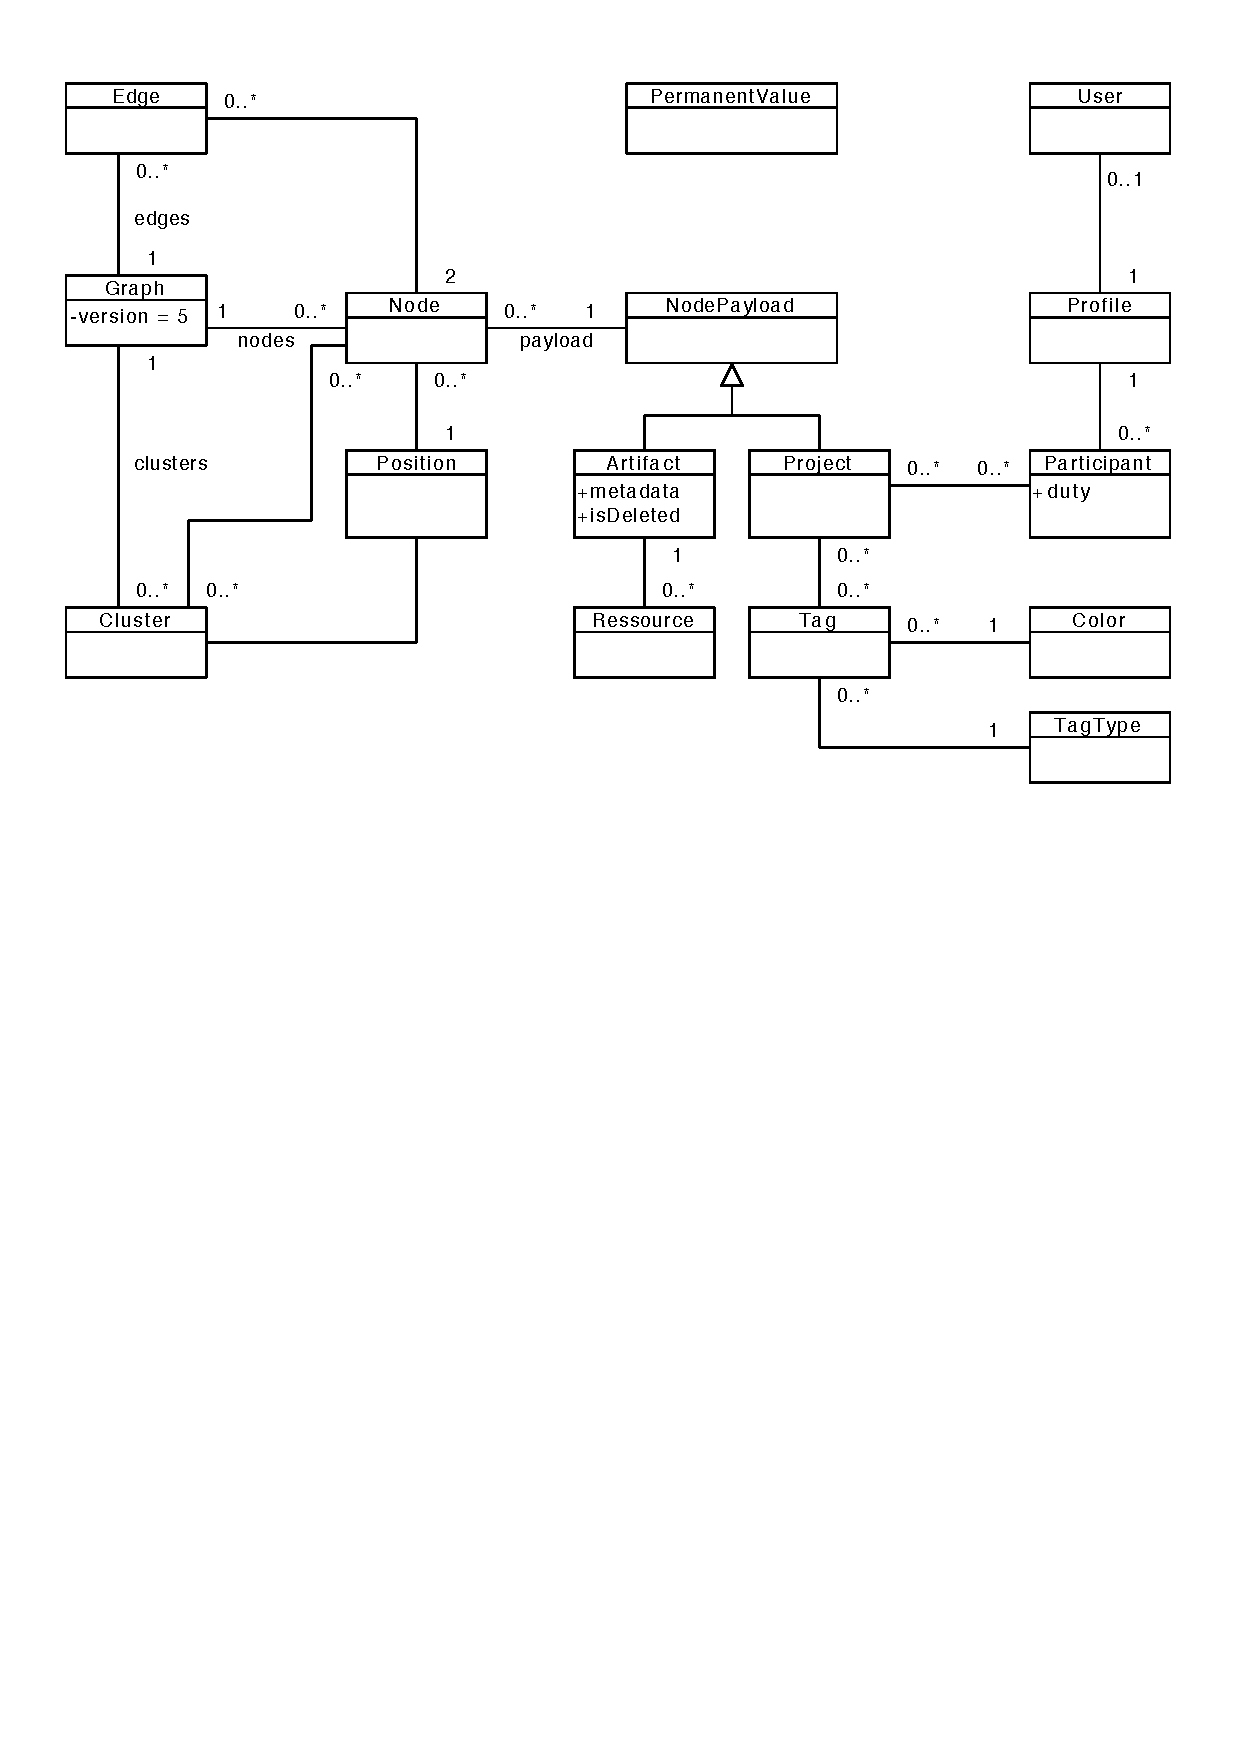
\includegraphics[width=1.0\textwidth]{img/complete_model.pdf}  
   \caption{Datenmodell von Project-Zoom}
  \label{fig:complete-model} 
\end{figure}
\pagebreak
\section{Objektdiagramm für einen beispielhaften Graphen}
\begin{figure}[h!t]
  \centering     
  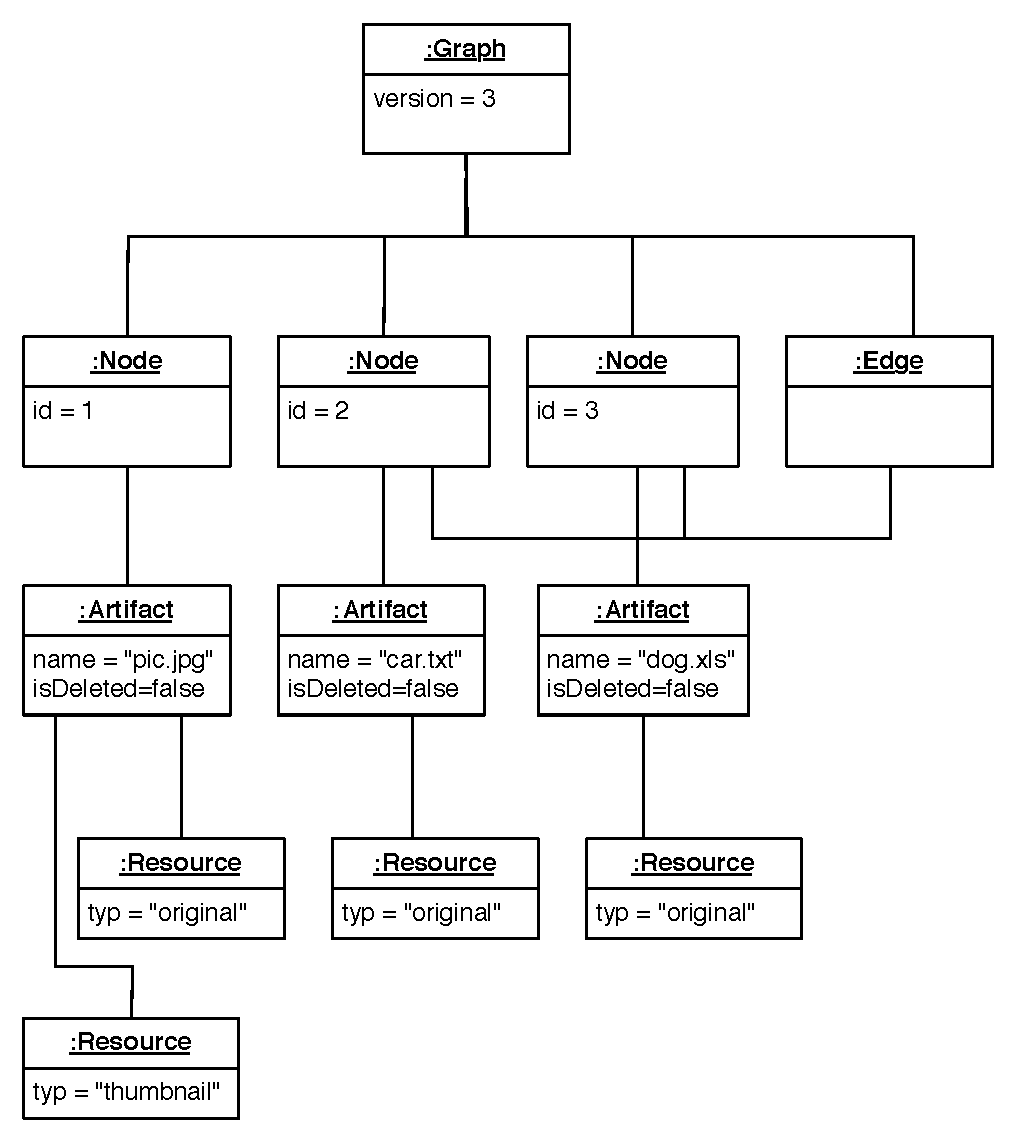
\includegraphics[width=0.8\textwidth]{img/instanz_graph.pdf}  
   \caption{Objektdiagramm eines beispielhaften Graphen. Zur Wahrung der Übersichtlichkeit ist die Position jedes Nodes nicht als Objekt visualisiert.}
  \label{fig:graph-bsp} 
\end{figure}
 
\section{InfoQ Umfrage zu Webframeworks der JVM}
In der Tabelle in der Abbildung \ref{fig:infoq-survey} sind die Umfrageergebnisse der InfoQ-Umfrage mit 1894 Teilnehmern von der Seite \url{http://www.infoq.com/research/jvm-web-frameworks.auf} zum angegebenen Zeitpunkt zu sehen.
\begin{figure}[ht]  
  \centering     
  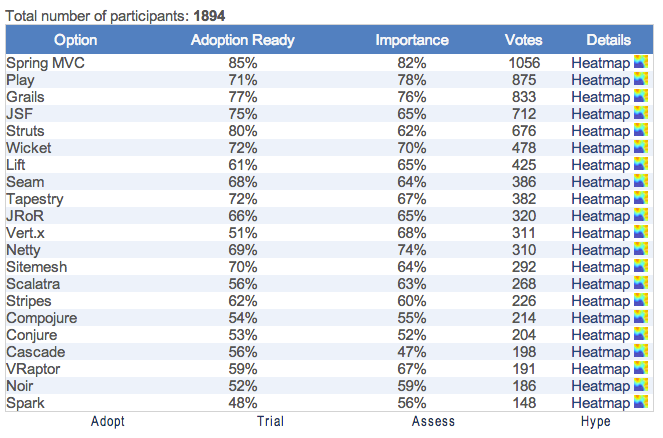
\includegraphics[width=1.0\textwidth]{img/infoq.png}  
   \caption{Stand der Umfrage am 26. Juni 2013}
  \label{fig:infoq-survey} 
\end{figure}

\section{Performance Test}
\label{sec:performance-test}
Project-Zoom wurde mit den folgenden Einstellungen für Apache Bench getestet:
\begin{lstlisting}
ab -g output100.txt -c 10 -n 100000 http://localhost:9000/projects
\end{lstlisting}

Weiterhin wurde noch ein Session-Cookie übergeben, um auf die geschütze Ressource zugreifen zu dürfen. Die Ergebnisse sind in den Abbildungen \ref{fig:perf1} und \ref{fig:perf2} zu sehen. Die Grafiken wurden mit Hilfe von \url{https://loadosophia.org} erstellt.

\begin{figure}
  \centering     
  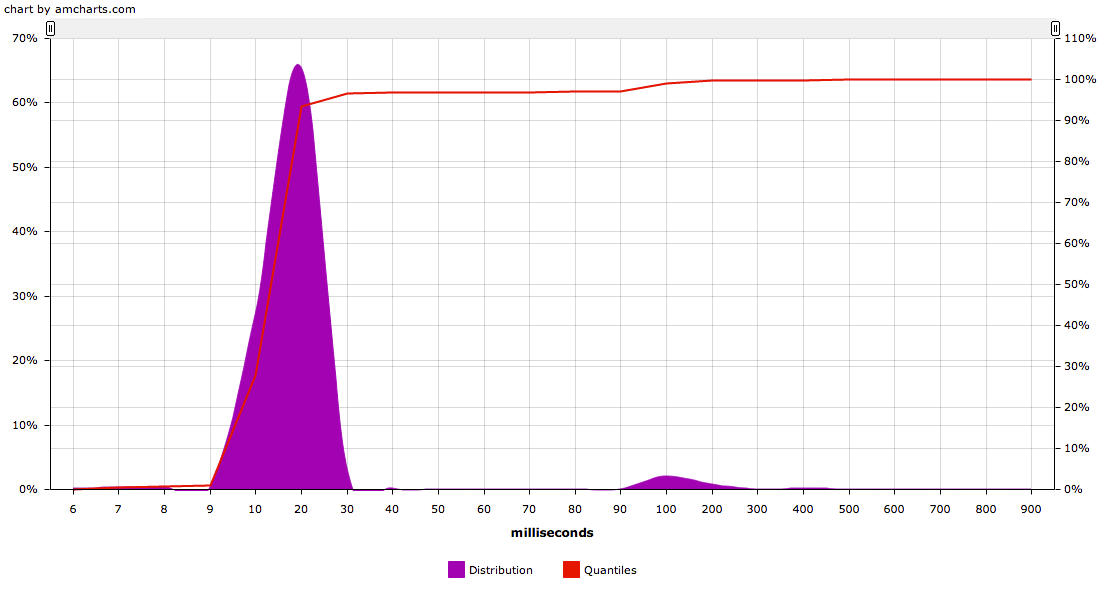
\includegraphics[width=1.0\textwidth]{img/perf1.png}  
   \caption{Dichte- und Verteilungsfunktion der Antwortzeiten }
  \label{fig:perf1} 
\end{figure}

\begin{figure}  
  \centering     
  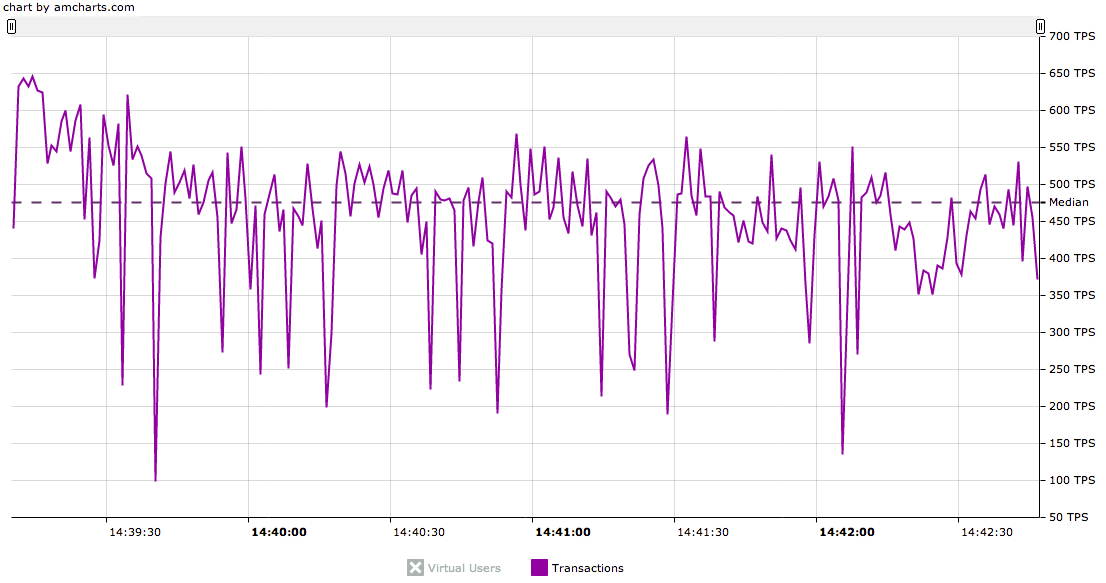
\includegraphics[width=1.0\textwidth]{img/perf2.png}  
   \caption{Durchsatz in abgeschlossenen Übertragungen pro Sekunde über die Zeit}
  \label{fig:perf2} 
\end{figure}


\section{Überblick über die vorhandenen Events}
\label{event-overiview}
In der Tabelle \ref{tab:events} sind alle Events zu sehen, die mit dem Backend-Core interagieren.

\begin{table}
    \begin{tabular}{|l|l|p{4.8cm}|}
    \hline
    ~                   & Parameter                                                                & Bedeutung                                                  \\ \hline
    ArtifactFound       & \begin{lstlisting}[gobble=4] 
    originalStream: InputStream
    artifact: ArtifactLike
    \end{lstlisting}                      & Artefakt von Konnektor gefunden                            \\ \hline
    ArtifactDeleted     & \begin{lstlisting}[gobble=4]
    artifact: ArtifactLike
    \end{lstlisting}                                                   & Löschung von Artefakt durch Konnektor festgestellt         \\ \hline
    ArtifactAggregation & \begin{lstlisting}[gobble=4]
    _project: String
    l: List[ArtifactFound]
    \end{lstlisting}                                 & Auflistung aller Artefakte eines Projektes durch Konnektor \\ \hline
    ArtifactRenamed     & \begin{lstlisting}[gobble=4]
    artifact: ArtifactLike
    name: String
    \end{lstlisting}                                     & Umbenennung von Artefakt durch Konnektor festgestellt      \\ \hline
    ArtifactMoved       & \begin{lstlisting}[gobble=4]
    artifact: ArtifactLike
    path: String
    \end{lstlisting}                                     & Verschiebung von Artefakt durch Konnektor festgestellt     \\ \hline
    ResourceFound       & \begin{lstlisting}[gobble=4]
    inputStream: InputStream
    artifact: ArtifactLike
    resource: ResourceLike
    \end{lstlisting} & Neue Resource für Artefakt gefunden                        \\ \hline
    ArtifactUpdated     & \begin{lstlisting}[gobble=4]
    artifact: ArtifactLike
    \end{lstlisting}                                                   & Artefakt in der DB geändert                                \\ \hline
    ArtifactInserted    & \begin{lstlisting}[gobble=4]
    artifact: ArtifactLike    
    \end{lstlisting}                                               & Artefakt zur DB hinzugefügt                                \\ \hline
    ResourceUpdated     & \begin{lstlisting}[gobble=4]
    file: File
    artifact: ArtifactLike
    resource: ResourceLike
    \end{lstlisting}               & Resource in der DB geändert                                \\ \hline
    ResourceInserted    & \begin{lstlisting}[gobble=4]
    file: File
    artifact: ArtifactLike
    resource: ResourceLike
    \end{lstlisting}               & Resource zur DB hinzugefügt                                \\ \hline
    ProjectFound        & \begin{lstlisting}[gobble=4]
    project: ProjectLike
    \end{lstlisting}                                                     & Projekt von Konnektor gefunden                             \\ \hline
    ProjectAggregation  & \begin{lstlisting}[gobble=4]
    l: List[ProjectFound]      
    \end{lstlisting}                                               & Auflistung mehrerer gefundener Projekte                    \\ \hline
    ProfileFound        & \begin{lstlisting}[gobble=4]
    profile: Profile   
    \end{lstlisting}                                                       & Profil von Konnektor gefunden                              \\ \hline
    ProfileAggregation  & \begin{lstlisting}[gobble=4]
    l: List[ProfileFound]  
    \end{lstlisting}                                                   & Auflistung mehrerer gefundener Profile                     \\ \hline
    GraphUpdated        & \begin{lstlisting}[gobble=4]
    graph: Graph
    patch: JsValue
    \end{lstlisting}                                             & Graph in der DB mit Patch geändert                         \\ \hline
    \end{tabular}
    \caption{Übersicht über Events des Backend-Core}
    \label{tab:events}
\end{table}

\textsc{ArtifactActor}
\begin{labeling}{\textbf{Subscription f{\"u}r:}}
  \item[Publishes] ArtifactUpdated, ArtifactInserted, ResourceUpdated, ResourceInserted
  \item[Subscription f{\"u}r] ArtifactFound, ArtifactDeleted, ArtifactAggregation, ArtifactRenamed, ArtifactMoved, ResourceFound
\end{labeling}

\textsc{KnowledgeActor}
\begin{labeling}{\textbf{Subscription f{\"u}r:}}
  \item[Subscription f{\"u}r] ProjectFound, ProjectAggregation, ProfileFound, ProfileAggregation
\end{labeling}

\textsc{Konnektoren}
\begin{labeling}{\textbf{Subscription f{\"u}r:}}
  \item[Publishes] ProfileAggregation, ProjectAggregation, ArtifactFound, ArtifactRenamed, ArtifactMoved, ArtifactDeleted, ArtifactAggregation
\end{labeling}

\textsc{Thumbnailgenerator}
\begin{labeling}{\textbf{Subscription f{\"u}r:}}
  \item[Publishes] ResourceFound
  \item[Subscription f{\"u}r] ResourceInserted, ResourceUpdated
\end{labeling}

\appendixChapter{REST-Schnittstelle}
\label{sec:rest-interaface}
    %!TEX root = ../../Bachelorarbeit.tex
\appendixChapter{Interviewprotokolle}
\label{app:TODO2}

	\end{appendix}
	
	%%%%%%%%%%%%%%%%%%%%%%%%%%%%%%%%%%%%%%%%%%%%%%%%%%%%%%%%%%%%%
	%% STATURATION DECLARATION
	%%%%%%%%%%%%%%%%%%%%%%%%%%%%%%%%%%%%%%%%%%%%%%%%%%%%%%%%%%%%%
	\chapter*{Eidesstattliche Erkl\"arung}
\clearscrheadfoot

Ich erkl\"are hiermit, dass ich die vorliegende Arbeit selbstst\"andig verfasst und daf\"ur keine
anderen als die genannten Quellen und Hilfsmittel verwendet habe.

\begin{flushleft}
\vspace{3cm}
\docAuthor
\end{flushleft}
\begin{flushleft}
\selectlanguage{german}
\docCity{} \docDate
\end{flushleft}

\end{document}
%%%%%%%%%%%%%%%%%%%%%%%%%%%%%%%%%%%%%%%%%%%%%%%%%%%%%%%%%%%%%
%% END DOKUMENT
%%%%%%%%%%%%%%%%%%%%%%%%%%%%%%%%%%%%%%%%%%%%%%%%%%%%%%%%%%%%%